
\section{Challenges in Large-scale Spectrum Measurements}

Power measurements for wireless spectrum in the Cellular and Wi-Fi frequency bands are highly dependent on the concentration of mobile devices (smartphones, tablets etc.).
 Consequently, these measurements exhibit strong temporal and spatial variation, governed by the mobility of users, the variety in types of devices and associated service providers.
 Studying the types of devices, most devices support multiple cellular frequencies and almost always support Wi-Fi at 2.4 GHz (newer devices also support Wi-Fi at 5 GHz).
 The support for multiple cellular frequencies in mobile devices is driven largely by the incompatible frequency bands used by the service providers.
 The Cellular Telecommunications and Internet Association (CTIA) \cite{CTIA} \cite{wiki:LTEBands} lists more than 20 facility-backed wireless service providers who operate their services in different frequency bands with only few bands overlapping across multiple providers.

\subsubsection{What cellular frequencies should we choose to study?} \label{subsubsec:whatfreq}
Table \ref{table:SpectrumAllocation} shows the cellular frequency band allocations for the top five wireless providers in the US who collectively account for over 400 million subscribers.
 There are more than 50 virtual operators which use the networks of these facility-backed wireless providers to provide service \cite{wiki:LTEBands}.
 As a result, it seems reasonable to confine this analysis of the cellular spectrum to the frequency bands from Table \ref{table:SpectrumAllocation} as representative of the cellular spectrum usage.
 
\begin{table*}[t]
\centering
\caption{Cellular Frequency Band Allocation to the Top 5 Wireless Service Providers in the USA. \cite{wiki:LTEBands}}
\label{table:SpectrumAllocation}
\begin{tabular}{c}
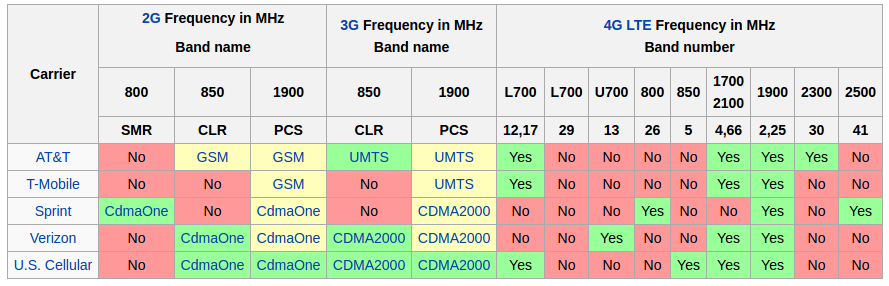
\includegraphics[width=\textwidth]{spectrum/tableSpectrumAllocation.png}
\end{tabular}
\end{table*}


\subsubsection{What are the challenges in city-wide measurement of wireless spectrum?}
For modeling these power measurements, RF propagation models are typically used to generate a power estimate.
 However, this technique lacks accuracy in city settings since buildings and multipath effects introduce complications in the model.
 Using detailed 3D terrain and building data, some authors have proposed to improve the modeling estimates \cite{RFModelsCity1} \cite{RFModelsCity2}.
 However, such approaches requires significant computational resources and modeling effort for generating power estimates.
 Additionally, some frequency bands show significant temporal variation in power as described in \cite{SpectrumDynamics} rising from the dynamics of users carrying mobile devices.
 Using RF propagation models would not capture such local, temporal variations of the spectral power inside a city, since the methods rely on the power output from the transmit antenna and ray-tracing simulations.


My goal here is to discuss a method to study temporal variations in spectrum usage that uses, comparitively, much lesser computational resources while simulatenously providing more accurate measurements than propagation models.

\subsubsection{Can opportunistic spectrum measurements help understand temporal variations?}
To address inaccuracy issues with RF propagation models, Zhang and Banerjee \cite{ZhangThesis} \cite{VScope} \cite{VScope2} propose VScope, an opportunistic spectrum sampling method to obtain ground truth power measurements, which can serve as "anchor" points to improve modeling accuracy for TV whitespace spectrum.
 VScope involves collecting measurements from a spectrum analyzer placed in a moving public transit vehicle.
 This method has the advantage of not requiring complicated terrain or building models to generate the power estimates.
 Instead, VScope chooses to use empirical data to correct estimates from RF propagation models.
 By augmenting such "ground truth" measurements combined with diversity in measurement locations (as a result of the moving vehicle on which the spectrum analyzer is mounted), VScope is able to improve the accuracy of the power estimates with a less computationally intensive approach.
 My work builds on top of the results from VScope and uncovers temporal variations from sparse measurements.


The VScope data has been collected for a 6 month period from July 2015 - January 2016 and has samples covering the entire city of Madison.
 Data has been collected for the frequency range 300 MHz - 3 GHz with a precision of 4 kHz in the frequency domain.
 It takes the spectrum analyzer approximately 7 minutes to do a full sweep of measurements from 300 MHz - 3 GHz (the complete frequency range for measurement).
 These measurements include the frequencies of interest as identified in Section \ref{subsubsec:whatfreq}.

I define sparsity of measurements here as less than 5 power measurements for a given frequency band within a given hour of the day at any location within a city.
 The opportunistic spectrum measurements from VScope are sparse by nature; the sparsity is induced by the varying routes, schedules and motion of the public transit vehicle.
 It is possible to identify three types of sparsity in the VScope data, as listed below.

\paragraph{Motion Induced Sparsity} Because of the motion of the bus and the 7 minute interval it takes the spectrum analyzer to sweep the entire frequency range of measurement, a given location has very few samples within any one hour period.
 Additionally, the samples so collected only correspond to a small portion of the complete frequency range (the measurements recorded while the transit vehicle is in the "vicinity" of the location).

\paragraph{Schedule Induced Sparsity} The vehicle carrying the spectrum analyzer is typically assigned to a single route for a specific day.
 However, the times during which the vehicle actually passes through a given location depends on both traffic conditions and schedules assigned by the transit authority.
 Consequently, a given location has measurements recorded only at certain hours within a single day.

\paragraph{Route Induced Sparsity} The vehicle carrying the spectrum analyzer is regularly reassigned to different transit routes within the city.
 Consequently, when it's required to analyze weekly, monthly or seasonal trends at a single location, the number of measurements is low in number across different days.\\

Owing to this sparsity, the data provides us partial information about temporal variation of spectral power, at a given location.
 Because of the missing samples, the data cannot be used "as is" to study temporal variations.

\subsubsection{How do we address the sparsity in spectrum measurement?} \label{subsubsec:KeyIdea}

\textbf{Key Intuition:} Given that only cellular and Wi-Fi frequencies are being studied, my conjecture is that the samples collectively show strong linear relationships.
 This intuition stems from two factors:
\begin{itemize}
\item The mobile devices that cause local variations in the spectral power are typically active in multiple frequency bands at the same time. For example, smartphones (that form a large share of common mobile devices) are typically active in both the 4G LTE bands as well as the Wi-Fi bands.
\item The circadian rhythms of people moving through a particular location causes repetitions or simple linear patterns in temporal variations. For example, a large majority of people work 9 to 5 jobs and are likely to cross the same location twice a day (repetition).
\end{itemize}

Therefore, we can use this simplying assumption of linear relationships between spectrum measurements to estimate the missing samples from the observed samples.

\subsubsection{Can we collect better data? Or is the sparsity unavoidable?}

The motion induced sparsity is especially interesting because it is caused, in large part, owing to the 7 minute interval the spectrum analyzer takes to do one full sweep of the frequency range.
 Therefore, an improvement in the measurement cycle with better instrumentation can significantly decrease the sparsity induced resulting from the motion of the public transit vehicle, which in turn would help build better temporal models.

In contrast, the sparsity in measurements induced by the varying routes and schedules of the public transit vehicle are uncontrollable factors and have to be treated as an inherent sparsity in the measurements.
 This stems from the fact that we deployed only one spectrum analyzer in a single public transit vehicle.
 If we had multiple spectrum analyzers deployed in multiple vehicles, this sparsity would be reduced.
 However, deploying multiple spectrum analyzers comes with the overhead of increased cost since such high resolution spectrum analyzers are quite expensive.
 Consequently, the Schedule and Route induced sparsities can be attributed to a trade-off between deployment cost and quality of data.

A completely different angle to solve this would be to employ solutions such as WiSee \cite{WiSee} which bring the capabilities of a spectrum analyzer to the smartphone.
 Such an approach would allow for crowdsourced acquisition of spectrum measurements which could potentially provide data with much lower sparsity, depending on the adoption of the approach.
 Even in this scenario, we believe that the methodology discussed in this chapter could prove valuable in estimating temporal variation in spectrum measurements.

